%----------------------------------------------------------------------------------------
%	PACKAGES AND OTHER DOCUMENT CONFIGURATIONS
%----------------------------------------------------------------------------------------
\documentclass[xcolor=dvipsnames]{beamer}

\usepackage[scale=1.24]{beamerposter} % Use the beamerposter package for laying out the poster
\usepackage{graphicx}
\usepackage{multirow}

\usepackage{array}
\usepackage{tabu}

\usetheme{confposter} % Use the confposter theme supplied with this template

\definecolor{cadet}{rgb}{0.33, 0.41, 0.47}
\definecolor{cadetgrey}{rgb}{0.57, 0.64, 0.69}
\definecolor{bostonunivred}{rgb}{0.9, 0.0, 0.0}
\definecolor{aliceblue}{rgb}{0.94, 0.97, 1.0}
\setbeamercolor{block title}{fg=cadet,bg=white} % Colors of the block titles
\setbeamercolor{block body}{fg=black,bg=white} % Colors of the body of blocks
\setbeamercolor{block alerted title}{fg=white,bg=cadetgrey} % Colors of the highlighted block titles
\setbeamercolor{block alerted body}{fg=black,bg=dblue!10} % Colors of the body of highlighted blocks
% Many more colors are available for use in beamerthemeconfposter.sty

%-----------------------------------------------------------
% Define the column widths and overall poster size
% To set effective sepwid, onecolwid and twocolwid values, first choose how many columns you want and how much separation you want between columns
% In this template, the separation width chosen is 0.024 of the paper width and a 4-column layout
% onecolwid should therefore be (1-(# of columns+1)*sepwid)/# of columns e.g. (1-(4+1)*0.024)/4 = 0.22
% Set twocolwid to be (2*onecolwid)+sepwid = 0.464
% Set threecolwid to be (3*onecolwid)+2*sepwid = 0.708

\setlength\parindent{24pt}
\newlength{\sepwid}
\newlength{\onecolwid}
\newlength{\twocolwid}
\newlength{\threecolwid}
\setlength{\paperwidth}{48in} 
\setlength{\paperheight}{36in}
\setlength{\sepwid}{0.024\paperwidth} % Separation width (white space) between columns
\setlength{\onecolwid}{0.22\paperwidth} % Width of one column
\setlength{\twocolwid}{0.464\paperwidth} % Width of two columns
\setlength{\threecolwid}{0.708\paperwidth} % Width of three columns
\setlength{\topmargin}{-0.5in} % Reduce the top margin size
%-----------------------------------------------------------

\usepackage{graphicx} 
\usepackage{booktabs} 

%----------------------------------------------------------------------------------------
%	TITLE SECTION 
%----------------------------------------------------------------------------------------

\title{Predicting Florida Presidential Election Vote Shares} % Poster title

\author{{\huge Sam Yard}} % Author(s)


%----------------------------------------------------------------------------------------

\begin{document}

\addtobeamertemplate{block end}{}{\vspace*{2ex}} % White space under blocks
\addtobeamertemplate{block alerted end}{}{\vspace*{2ex}} % White space under highlighted (alert) blocks

\setlength{\belowcaptionskip}{2ex} % White space under figures
\setlength\belowdisplayshortskip{2ex} % White space under equations

\begin{frame}[t] % The whole poster is enclosed in one beamer frame

\begin{columns}[t] % The whole poster consists of three major columns, the second of which is split into two columns twice - the [t] option aligns each column's content to the top

\begin{column}{\sepwid}\end{column} % Empty spacer column

\begin{column}{\onecolwid} % The first column

%----------------------------------------------------------------------------------------
%	OBJECTIVES
%----------------------------------------------------------------------------------------

\begin{alertblock}{Research Question}
\begin{itemize}
\item[\textcolor{black}{\textbullet}] How do demographic factors, such as population by race, median income, and median housing prices, relate to the 2020 election outcomes in \textbf{Florida} counties?
\item[\textcolor{black}{\textbullet}]  This study investigates the connection between demographic characteristics in Florida counties and their \textbf{political preferences during the 2020 elections}. Florida, known for its diversity and political significance, has historically played a pivotal role in national elections, making it an ideal focal point for this analysis. 
\item[\textcolor{black}{\textbullet}] The research utilizes county-level election results and demographic data from the American Community Survey to provide comprehensive insights into the influence of demographics on election outcomes in Florida.
\end{itemize}
\end{alertblock}

%----------------------------------------------------------------------------------------

\begin{block}{Hypothesis Testing}
\textbf{Linear Model: } \newline
$dem\_votes \sim pop\_poc$ 
\begin{itemize}
\item [\textcolor{black}{\textbullet}] The null hypothesis for the coefficient associated with the variable $pop\_poc$ is: \\
$H_0: \beta_{pop\_poc} = 0$
\item [\textcolor{black}{\textbullet}] Associated Model Results:
\end{itemize}


\begin{tabular}{ |p{5.4cm}|p{5.5cm}|p{5cm}|p{4.5cm}|p{5cm}|}

 \hline
 \multicolumn{5}{|c|}{dem\_votes $\sim$ pop\_poc} \\
 \hline
 & Estimate &Std.Error &t-value & Pr(>|t|)\\
 \hline
 Intercept   & 3.292e+0    &1.557&   21.146 & < 2e-16\\
 \hline
 $pop\_poc$ &   1.977e-05  & 4.265e-06   &4.635 & 1.77e-05\\
 \hline
\end{tabular}

\begin{quote}
\textcolor{white}{\textbullet}This model was employed to investigate the relationship between the Democratic vote share in the 2020 presidential elections, and the percentage of the population that is people of color. $H_0$ suggests no impact of the population of people of color on Democratic vote share. However, the estimated coefficient was found to be statistically significant, providing evidence against $H_0$. The coefficient indicates that an increase in the population of people of color is associated with a corresponding increase in Democratic vote share.
\end{quote}
\end{block}

%------------------------------------------------

\end{column} % End of the first column
\begin{column}{\sepwid}\end{column} % Empty spacer column
\begin{column}{\twocolwid} % Begin a column which is two columns wide (column 2)
\begin{columns}[t,totalwidth=\twocolwid] % Split up the two columns wide column
\begin{column}{\onecolwid}\vspace{-.6in} % The first column within column 2 (column 2.1)

%----------------------------------------------------------------------------------------

\begin{block}{Hypothesis Testing Cont.}

\begin{itemize}
\textbf{Linear Model:} 

$rep\_votes \sim median\_housing\_price$ \\ \newline
\item[\textcolor{black}{\textbullet}] The null hypothesis for the coefficient associated with the variable $median\_housing\_price$ is: \\
$$H_0: \beta_{median\_housing\_price} = 0$$
\item[\textcolor{black}{\textbullet}]Associated Model Results:

\end{itemize}    

\newline
\newline
\begin{tabular}{ |p{5.2cm}|p{5.9cm}|p{5cm}|p{4.2cm}|p{5cm}|}

 \hline
 \multicolumn{5}{|c|}{$rep\_votes \sim median\_housing\_price (mhp)$} \\
 \hline
 & Estimate &Std.Error &t-value & Pr(>|t|)\\
 \hline
 Intercept   & -2.806e+04    &2.688e+04&   -1.044  & 0.3\\
 \hline
 $mhp$ &   6.129e-01  &1.329e-01   &4.612 & 1.93e-05\\
 \hline
\end{tabular}
\newline

\begin{quote}
\textcolor{white}{\textbullet}This model reveals a significant positive correlation between median housing prices and Republican (0.613, p < 0.00001) votes. These findings suggest that housing affordability, reflected in median prices, may influence political preferences. The interplay of socio-economic factors in shaping electoral dynamics is evident. However, caution is warranted, as correlation does not imply causation. Further research considering additional variables is crucial for a comprehensive understanding of the relationship between housing prices and political preferences in Florida counties.



\end{quote}

\end{block}


\begin{block}{2020 Vote Shares}
\begin{figure}
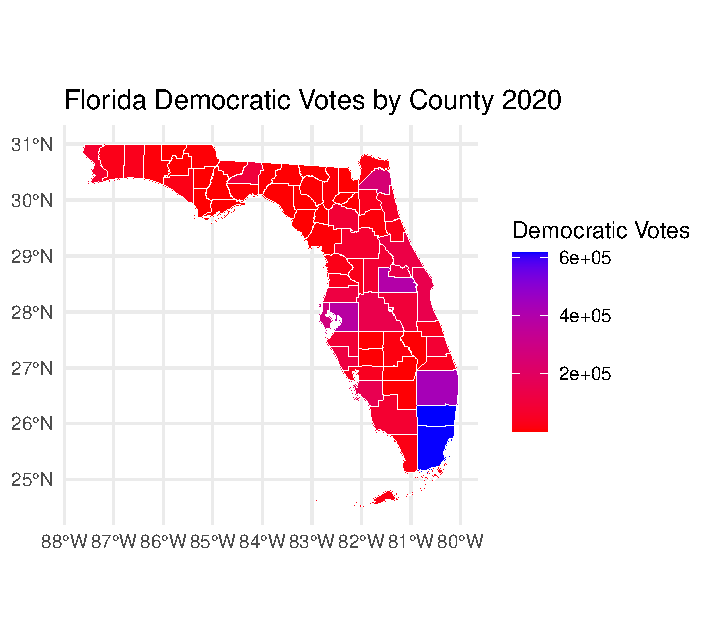
\includegraphics[trim={1.45cm 1cm 1.25cm 1cm},clip,scale=2.7]{dem_votes2020.pdf}
\caption{Florida Vote Share by County 2020}
\end{figure}
\end{block}
\end{column} % End of column 2.1
\begin{column}{\onecolwid}\vspace{-.6in} % The second column within column 2 (column 2.2)

%----------------------------------------------------------------------------------------
%	METHODS
%----------------------------------------------------------------------------------------

\begin{block}{Demographic Impact}

\begin{figure}
\includegraphics[trim={0.2cm 0.2cm 0.5cm 0.8cm},clip,scale=1.9]{race_voteshare.pdf}
\caption{White population vs. 2020 Presidential vote share}
\end{figure}


\begin{tabular}{ |p{5.2cm}|p{5.9cm}|p{5cm}|p{4.2cm}|p{5cm}|}

 \hline
 \multicolumn{5}{|c|}{Average Demographics of Bottom 5 Counties} \\
 \hline
 & Dem Vote Share &White Pop &PoC Pop & House Cost\\
 \hline
 Bottom 5 counties   & 14.414\%    &78.54\%&   21.46\% & \$110,500\\
 \hline

\end{tabular}
\newline
\newline
Bottom Five Counties: Holmes, Lafayette, Baker, Dixie, Union
\newline
\begin{tabular}{ |p{5.2cm}|p{5.9cm}|p{5cm}|p{4.2cm}|p{5cm}|}

 \hline
 \multicolumn{5}{|c|}{Average Demographics of Top 5 Counties} \\
 \hline
 & Dem Vote Share &White Pop &PoC Pop & House Cost\\
 \hline
 Bottom 5 counties   & 63.86\%    &40.01\% &  59.99\%  & \$210,560\\
 \hline

\end{tabular}
\newline
\newline
Bottom Top Counties: Gadsen, Broward, Leon, Alachua, Orange

\begin{quote}
The top five counties in Florida exhibit a strong Democratic vote share, and reflects a diverse population composition with 59.99\% People of Color. These counties also feature a relatively higher median housing price of \$210,560. In contrast, the bottom five counties have a lower Democratic vote share of 14.41\%, a predominantly White population (78.54\%), and a more affordable median housing price of \$110,500. These findings suggest a correlation between political preferences, racial diversity, and housing affordability in Florida counties. However, a comprehensive understanding would require consideration of additional factors and context.
\end{quote}
\end{block}


%----------------------------------------------------------------------------------------

\end{column} % End of column 2.2

\end{columns} % End of the split of column 2 - any content after this will now take up 2 columns width

%----------------------------------------------------------------------------------------
%	IMPORTANT RESULT
%----------------------------------------------------------------------------------------



%----------------------------------------------------------------------------------------

\begin{columns}[t,totalwidth=\twocolwid] % Split up the two columns wide column again

%\begin{column}{\onecolwid} % The first column within column 2 (column 2.1)

%----------------------------------------------------------------------------------------
%	MATHEMATICAL SECTION
%----------------------------------------------------------------------------------------


%----------------------------------------------------------------------------------------

%\end{column} % End of column 2.1

%\begin{column}{\onecolwid} % The second column within column 2 (column 2.2)

%----------------------------------------------------------------------------------------
%	RESULTS
%----------------------------------------------------------------------------------------

%\begin{block}{Results}

%The cache compression coverage is grouped into low, medium, medium-high \& high coverage groups. The confusion matrix below evinces the performance of test set data true vs predictions.


%\end{block}

%----------------------------------------------------------------------------------------

%\end{column} % End of column 2.2

\end{columns} % End of the split of column 2

\end{column} % End of the second column

\begin{column}{\sepwid}\end{column} % Empty spacer column

\begin{column}{\onecolwid} % The third column



%----------------------------------------------------------------------------------------
%	CONCLUSION
%----------------------------------------------------------------------------------------

\begin{block}{Conclusions}\\
\begin{quote}
    The model findings suggest that demographic factors related to the population of people of color play a significant role in shaping Democratic electoral support, emphasizing the importance of considering such demographic dynamics in understanding and predicting political preferences in the studied region during the 2020 presidential elections and beyond.
\end{quote}
\newline
\begin{quote}
    For predicting future elections in Florida, recognizing the influence of socio-economic factors, particularly household income, may be crucial. Policymakers and analysts could consider these economic dynamics when devising strategies and forecasts. Nevertheless, the intricate nature of political choices underscores the need for a comprehensive understanding that incorporates various contributing factors.
\end{quote}

\end{block}

%----------------------------------------------------------------------------------------
%	ADDITIONAL INFORMATION
%----------------------------------------------------------------------------------------


%	CONTACT INFORMATION


\begin{alertblock}{Contact Information}

 • samyard@bu.edu

\end{alertblock}


\end{column} % End of the third column

\end{columns} % End of all the columns in the poster

\end{frame} % End of the enclosing frame

\end{document}
